%\documentclass{article}
%\usepackage{graphicx,subfigure}
%\begin{document}

\begin{figure}[!h]
  \centering
  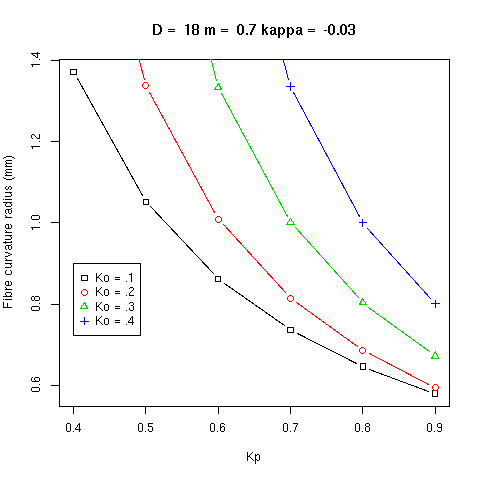
\includegraphics[width=1.0\textwidth]{RvsKpm7.png}
 \caption{Plot of fibre curvature calculated using equation~\ref{eqn:timowool} against $K_{p}$ , with a separate line shown for several values of $K_{o}$, and with the other parameters held constant at $D=18$, $m=0.7$.}
  \label{fig:curvkp40}
\end{figure}

%\end{document}

